\chapter{Desarrollo}
\thispagestyle{empty}

\section{Descripción del capítulo} \label{sec:\thesection}
En este capitulo se desarrollarán las soluciones propuestas en el capítulo de diseño. Esto implica detallar el proceso realizado, describir los cambios que se debieron hacer en caso de que el planteo inicial no haya funcionado, análisis de resultados, etc. \\
Cada sección será redactada en el orden que se hicieron, debido a que unas partes dependen de otras para poder desarrollarse.

\section{Firmware del updown - Librerías de bajo nivel} \label{sec:\thesection}

\subsection{DigitalIO}
El desarrollo del módulo de entradas y salidas digitales (DigitalIO) está basado en el capítulo 18 de la hoja de datos del Atmega328p. 

\textcolor{FIXME}{FIJATE SI NO ES MEJOR EMPEZAR POR LO DE QUE EL ACCESO SE HACE CON 3 FUNCIONES, Y DE AHI DECIR QUÉ HACE CADA FUNCIÓN}

\subsubsection{Uso}
En microcontroladores de la marca Atmel, como es el de este proyecto, las entradas y salidas digitales de manejan mediante 3 registros: el DDRn (Data Direction Register n), PORTn (Port n Data Register) y PINn (Port n Input Pins Address). La "n" en los registros se refiere al registro específico a ser accedido, que en el caso de este microcontrolador puede ser B, C o D.

Para configurar un pin, que es una pata del microcontrolador, como entrada o salida digital primero se elige la dirección del mismo, o sea, si se utilizará como entrada O como salida digital. Para esto se utiliza el registro DDRn, en donde escribir un bit de este registro en 1 significa configurar el pin asociado a este bit como salida o Output, mientras que si se escribe en 0 significa configurar al pin como entrada o Input. \\
Si el pin fue configurado como salida se setea su valor mediante el registro PORTn. Un 1 en un bit de este registro significa poner en HIGH (5 Volts) la salida asociada a ese bit, mientras que un 0 es un estado LOW (0 Volts).\\
Si el pin fue configurado como entrada se lee su valor del registro PINn, que puede ser 0 o 1 (HIGH o LOW). A un pin configurado como entrada se le puede, además, habilitar una resistencia pull-up interna del microcontrolador, haciendo que por defecto el canal esté en 1. El pull-up se encuentra deshabilitado por defecto, pero puede ser habilitado escribiendo un 1 en el bit análogo del registro PORTn.\\
Por ejemplo, si se quiere configurar el bit 3 del puerto B como entrada con pull-up y el bit 6 del puerto D como entrada en lenguaje C, se tiene:

\begin{lstlisting}[style=CStyle]
	/* --- Configuracion bit 3 puerto B como Input - Pullup --- */
	DDRB &= ~(1 << 3); // Configurcion como entrada
	PORTB |= (1 << 3); // Habilitacion pullup
	
	valorBit3PuertoB = PINB & (1 << 3); // Ejemplo lectura del bit
	
	/* --- Configuracion bit 6 puerto D como Output --- */
	DDRD |= (1 << 6); // Configurcion como salida
	
	PORTD |= (1 << 6); // Ejemplo escritura de un 1 en el bit
\end{lstlisting}

\subsubsection{Implementación}
El acceso al módulo se realiza a través de 3 funciones: una de inicialización (init), una de lectura (write) y otra de escritura (read), presentadas en la figura \ref{fig:3.1}. \\
Para facilitar la lecto-escritura y configuración de los pines se mapearon los bits de los puertos B,C y D a números, como se muestra en la tabla \ref{table:3.1}. El criterio de enumeración fue basado en los pines del Arduino UNO.

\begin{table}[!ht]
	\begin{center}
		\begin{tabular}{|c|c|c|}
			\hline
			\textbf{Puerto} & \textbf{Bit} & \textbf{Numero mapeado} \\
			\hline \hline
			D & 0, 1, 2, 3, 4, 5, 6, 7 & 0, 1, 2, 3, 4, 5, 6, 7 \\
			\hline
			B & 0, 1, 2, 3, 4, 5 & 8, 9, 10, 11, 12, 13 \\
			\hline
			C & 0, 1, 2, 3, 4, 5 & 14, 15, 16, 17, 18, 19\\
			\hline
		\end{tabular}
	\end{center}
	\caption{Mapeo de bits de los puertos a número}
	\label{table:\thetable}
\end{table}

\begin{figure}[!ht]
	\centering
	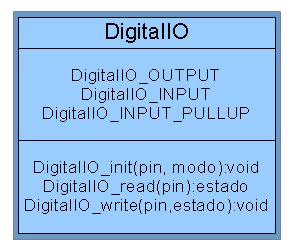
\includegraphics[width=6cm,scale=1]{resources/3_1-moduloDigitalIO.png}
	\caption{Diagrama del módulo DigitalIO}
	\label{fig:\thefigure}
\end{figure}



\subsection{ADC}
El desarrollo del módulo ADC está basado en el capítulo 28 de la hoja de datos del Atmega328p.

\subsubsection{Uso}

\subsubsection{Implementación}

\begin{figure}[!ht]
	\centering
	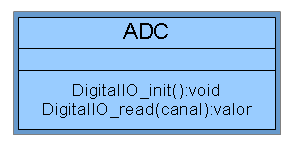
\includegraphics[width=6cm,scale=1]{resources/3_2-moduloADC.png}
	\caption{Diagrama del módulo ADC}
	\label{fig:\thefigure}
\end{figure}

\subsection{PWM}
El desarrollo del módulo PWM está basado en el capítulo 20 de la hoja de datos del Atmega328p.

\subsubsection{Uso}

\subsubsection{Implementación}

\subsection{EXINT}
El desarrollo del módulo de interrupciones externas (EXINT) está basado en el capítulo 17 y 18 de la hoja de datos del Atmega328p.

\subsubsection{Uso}

\subsubsection{Implementación}

\subsection{UART}
El desarrollo del módulo UART está basado en el capítulo 24 de la hoja de datos del Atmega328p.

\subsubsection{Uso}

\subsubsection{Implementación}

\subsection{SUART}
El desarrollo del módulo SUART está basado en el capítulo 19 de la hoja de datos del Atmega328p.

\subsection{Tick}
El desarrollo del módulo Tick está basado en el capítulo 22 de la hoja de datos del Atmega328p.

\subsubsection{Uso}

\subsubsection{Implementación}


\section{Controlador} \label{sec:\thesection}

\subsection{Relación entre cuentas de encoder y distancia}
Como se mencionó en la sección \ref{sec:2.3}, subsección 3, 

\subsection{Determinación de la velocidad máxima}

\subsection{Obtención del período de muestreo}
Como se mencionó en la sección \ref{sec:2.3}, subsección 3, 

\subsection{Obtención del modelo de la planta}

\subsection{Obtención del controlador}

\subsection{Ajuste del controlador}


\section{Dipswitch} \label{sec:\thesection}

\section{Firmware del updown - Librerías de alto nivel} \label{sec:\thesection}

\section{Firmware del updown - Función principal} \label{sec:\thesection}


